\subsubsection{\stid{3.14} ALExa}


\paragraph{Overview}

The ALExa project ({\sl Accelerated Libraries for Exascale}) focuses on
preparing the ArborX, DTK, Tasmanian, and ForTrilinos libraries for exascale
platforms and integrating these libraries into ECP applications.
These libraries deliver capabilities identified as needs of ECP applications:
%
(1) the ability the perform performance portable spatial searches between
arbitrary sets of distributed geometric objects (ArborX);
%
(2) the ability to transfer computed
solutions between grids with differing layouts on parallel accelerated
architectures, enabling multiphysics projects to seamlessly combine results
from different computational grids to perform their required simulations
(DTK); and
%
(3) the ability to construct fast and memory efficient surrogates to large
scale engineering models with multiple inputs and large number of outputs,
enabling uncertainty quantification (both forward and inverse) as well as
optimization and efficient multi-physics simulations in projects such as
ExaStar (Tasmanian); and
%
(4) the ability to interface large and complex Fortran-based codes to the
growing collection of Trilinos advanced solver capabilities that can
utilize next-generation platforms, the interface is done without C/C++
interface code (ForTrilinos).


These capabilities are being developed through ongoing interactions with our
ECP application project collaborators to ensure they will satisfy requirements
of these customers.  The libraries in turn take advantage of other ECP/SW
capabilities currently in development, including Trilinos and ForTrilinos,
Kokkos and SLATE.  The final outcome of the ECP project will be a set of
libraries deployed to facilities and also made broadly available as part of
the xSDK4ECP project.


{\bf ArborX}

{\it Purpose:} ArborX is an open-source library designed to provide
performance portable algorithms for geometric search.

{\it Significance:} General geometric search capabilities are needed in a wide
variety of applications including the generation of neighbor lists in
particle-based applications (e.g. molecular dynamics or general N-body
dynamics simulations) and mesh-mesh interactions including contact in
computational mechanics and solution transfer in multiphysics simulations.

{\it Performance portable search capabilities:} Shared memory and GPU
implementations of spatial tree construction; shared memory and GPU
implementations of various spatial tree queries; MPI front-end for
coordinating distributed spatial searches between sets of geometric objects
with different decompositions; communication plan generation based on spatial
search results.

{\it URL:} https://github.com/arborx/ArborX

{\bf DTK} (Data Transfer Kit)

{\it Purpose:} Transfers computed solutions between grids with differing
layouts on parallel accelerated architectures.

{\it Significance:} Coupled applications frequently have different grids with
different parallel distributions; DTK is able to transfer solution values
between these grids efficiently and accurately.

{\it Mesh and mesh-free interpolation capabilities:} multivariate data
interpolation between point clouds and grids; compactly supported radial basis
functions; nearest-neighbor and moving least square implementations; support
for standard finite-element shape functions and user-defined interpolants;
common applications include conjugate heat transfer, fluid structure
interaction, and mesh deformation.

{\it URL:} https://github.com/ORNL-CEES/DataTransferKit


{\bf Tasmanian} (Toolkit for Adaptive Stochastic Modeling and Non-Intrusive
Approximation)

{\it Purpose:} Constructs efficient surrogate models for high dimensional
problems and performs parameter calibration and optimization geared towards
applications in uncertainty quantification (UQ).

{\it Significance:} UQ pertains to the statistical properties of the output
from a complex model with respect to variability in multiple model inputs;
large number of simulations are required to compute reliable statistics which
is prohibitive when dealing with computationally expensive engineering
models. A surrogate model is constructed from a moderate set of simulations
using carefully chosen input values; analysis can then be performed on the
efficient surrogate.

{\it Sparse grids capabilities:} surrogate modeling and design of experiments
(adaptive multi-dimensional interpolation); reduced (lossy) representation of
tabulated scientific data; high dimensional numerical quadrature; data mining
and manifold learning.

{\it DiffeRential Evolution Adaptive Metropolis (DREAM) capabilities:}
Bayesian inference; parameter estimation/calibration; model validation.
global optimization and optimization under uncertainty.

{\it URL:} http://tasmanian.ornl.gov


{\bf ForTrilinos} (Fortran for Trilinos)

{\it Purpose:} ForTrilinos provides a seamless pathway for large and complex
Fortran-based codes to access Trilinos without C/C++ interface code.
This access includes Fortran versions of Kokkos abstractions for code
execution and data management..

{\it Significance:} The Exascale Computing Project (ECP) requires the successful
transformation and porting of many Fortran application codes in preparation for
ECP platforms. A significant number of these codes rely upon the scalable
solution of linear and nonlinear equations. The Trilinos Project contains
a large and growing collection of solver capabilities that can utilize
next-generation platforms, in particular scalable multicore, manycore,
accelerator and heterogeneous systems. Trilinos is primarily written in C++,
including its user interfaces. While C++ is advantageous for gaining access to
the latest programming environments, it limits Trilinos usage via Fortran.

{\it SWIG capabilities:}  an interface generator, SWIG, which the project is
extending, to create the object-oriented Fotran wrapper code that users can
access directly. This language translation will occur in both directions;
ForTrilinos will provide an inversion of control functionality that enables
custom extensions of the Trilinos solvers that are Fortran-based. Once the
ForTrilinos project is complete, a functional, extensible suite of capabilities
to access Trilinos on next-generation computing systems will be provided.

{\it URL:} https://github.com/trilinos/ForTrilinos

\paragraph{Key Challenges}

\indent

{\bf ArborX:} Search procedures to locate neighboring points, mesh cells, or
other geometric objects require tree search methods difficult to optimize on
modern accelerated architectures due to vector lane or thread divergence.

{\bf DTK:} General data transfer between grids of unrelated applications
requires many-to-many communication which is increasingly challenging as
communication to computation ratios are decreasing on successive HPC systems.
Maintaining high accuracy for the transfer requires careful attention to the
mathematical properties of the interpolation methods and is highly
application-specific.

{\bf Tasmanian:} Complex models usually have significant variability in
execution time for different model inputs, which leads to massive down-time
when employing the standard fork-join adaptive sparse grid algorithms.  After
the surrogate has been constructed, collecting the samples for statistical
analysis (or multi-physics simulations) requires a massive number of basis
evaluations and many sparse and dense linear operations.

{\bf ForTrilinos:} Developing the interfaces to the C++ libraries that provide
access to cutting-edge research, such as Trilinos,  is of significant benefit
to Fortran community. However, such interfaces must be well documented,
sustainable and extensible, which would require significant amount of resources
and investment. This is further complicated by the requirements to support
heterogeneous platforms (e.g., GPUs) and inversion-of-control functionality.
The manual approach to such interfaces has been shown to be unsustainable as it
requires interface developers to have in-depth expertise in  multiple languages
and the peculiarities in their interaction on top of the time commitment to
update the interfaces with changes in the library.

\paragraph{Solution Strategy}

\nobreak


\indent

{\bf ArborX:} ArborX builds on a Kokkos+MPI programming model to deploy to all
DOE HPC architectures. Extensive performance engineering has yielded
implementations that are both as performant in serial as state-of-the-art
libraries while also expanding on the capability provided by other libraries
by demonstrating thread scalability on both GPU and multi-core CPU
architectures..

{\bf DTK:} State-of-the-art, mathematically rigorous methods are used in DTK
to preserve accuracy of interpolated solutions.  Algorithms are implemented in
a C++ code base with extensive unit testing on multiple platforms.  Trilinos
packages are used to support interpolation methods.  Kokkos is used to achieve
performance portability across accelerated platforms.

{\bf Tasmanian:} Implement asynchronous DAG-based sparse grids construction
methods that preserve the convergence properties of the fork-join algorithms
but are insensitive to fluctuations in model simulation time.  Port the basis
evaluations and linear algebra to the GPU accelerators, and leverage the
SLATE/MAGMA capabilities to ensure performance portability across relevant
platforms.

{\bf ForTrilinos:} Develop a Fortran module for the Simplified Wrapper
Interface Generator (SWIG) utility~\cite{beazley1996swig}. SWIG is used to parse
C++ code and generate wrapper code, and was already used for this purpose for
several dozen target languages, most notably Python. The project took the
approach of adding a Fortran 2003 wrapper generator for SWIG in order to
fulfill many of the critical feature requirements for ForTrilinos.
The developed SWIG/Fortran functionality allowed to proceed with automatic
generation of Fortran interfaces to selected Trilinos libraries. The work is
conducted in phases, with each phase increasing the number of wrapped of
Trilinos packages.

%----------------------------------------

\paragraph{Recent Progress}

\indent

{\bf ArborX:} Extensive optimization work has yielded significant performance
improvements on accelerated and heterogeneous architectures. Recent results on
Summit show effective use of the Power9 hyperthreading capability as well as
excellent performance on the V100 GPU.

\begin{figure}[htb]
        \centering 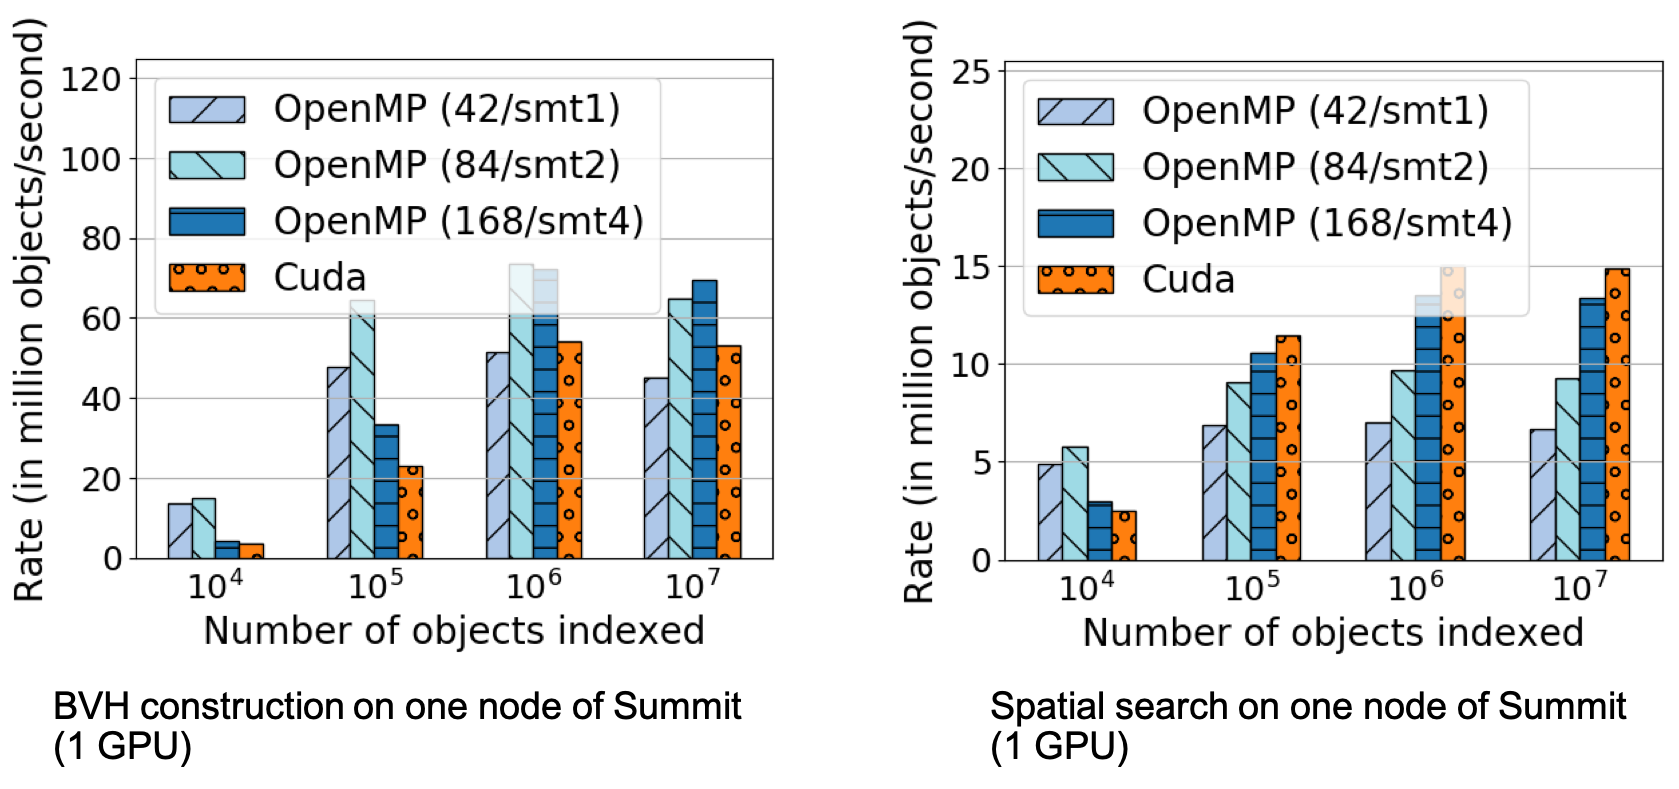
\includegraphics[width=3.0in]{projects/2.3.3-MathLibs/2.3.3.14-ALExa-ForTrilinos/arborx_summit.png} \caption{\label{fig:arborx-gpu}
        ArborX search performance on a single Summit node. One V100 GPU gives
        similar performance as the entire Power9 CPU performance on a node.}
\end{figure}

{\bf DTK:} Work with partner application ExaAM (WBS 2.2.1.05) created a
preliminary multiphysics driver capability for additive manufacturing
simulations using a parallel-in-time coupling strategy.

\begin{figure}[htb]
        \centering 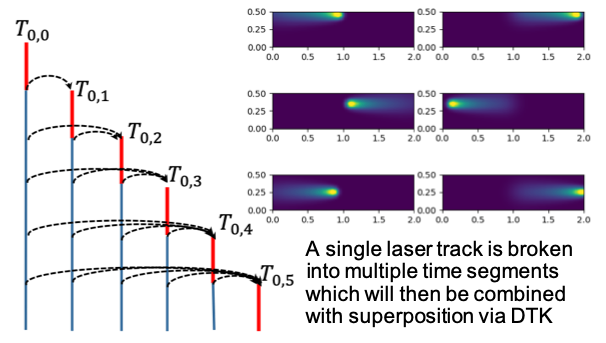
\includegraphics[width=3.0in]{projects/2.3.3-MathLibs/2.3.3.14-ALExa-ForTrilinos/dtk_exaam_pit.png} \caption{\label{fig:dtk-exaam-pit}
        New ExaAM parallel-in-time coupling. Each arrow represents a DTK
        transfer between different grids at different time points. Thousands
        of DTK maps will be used to interpolate and communicate information
        between steps. Image courtesy of Matt Bement (ExaAM Team) }
\end{figure}

{\bf Tasmanian:} The infrastructure of Tasmanian has been upgraded to support
the broader ECP focus of the work.  GPU acceleration of sparse grid surrogates
has been implemented.  Tasmanian recently enabled the ExaStar project to
reduce the size of a large-memory table of neutrino opacities by 10X while
still preserving accuracy.

\begin{figure}[htb]
        \centering
        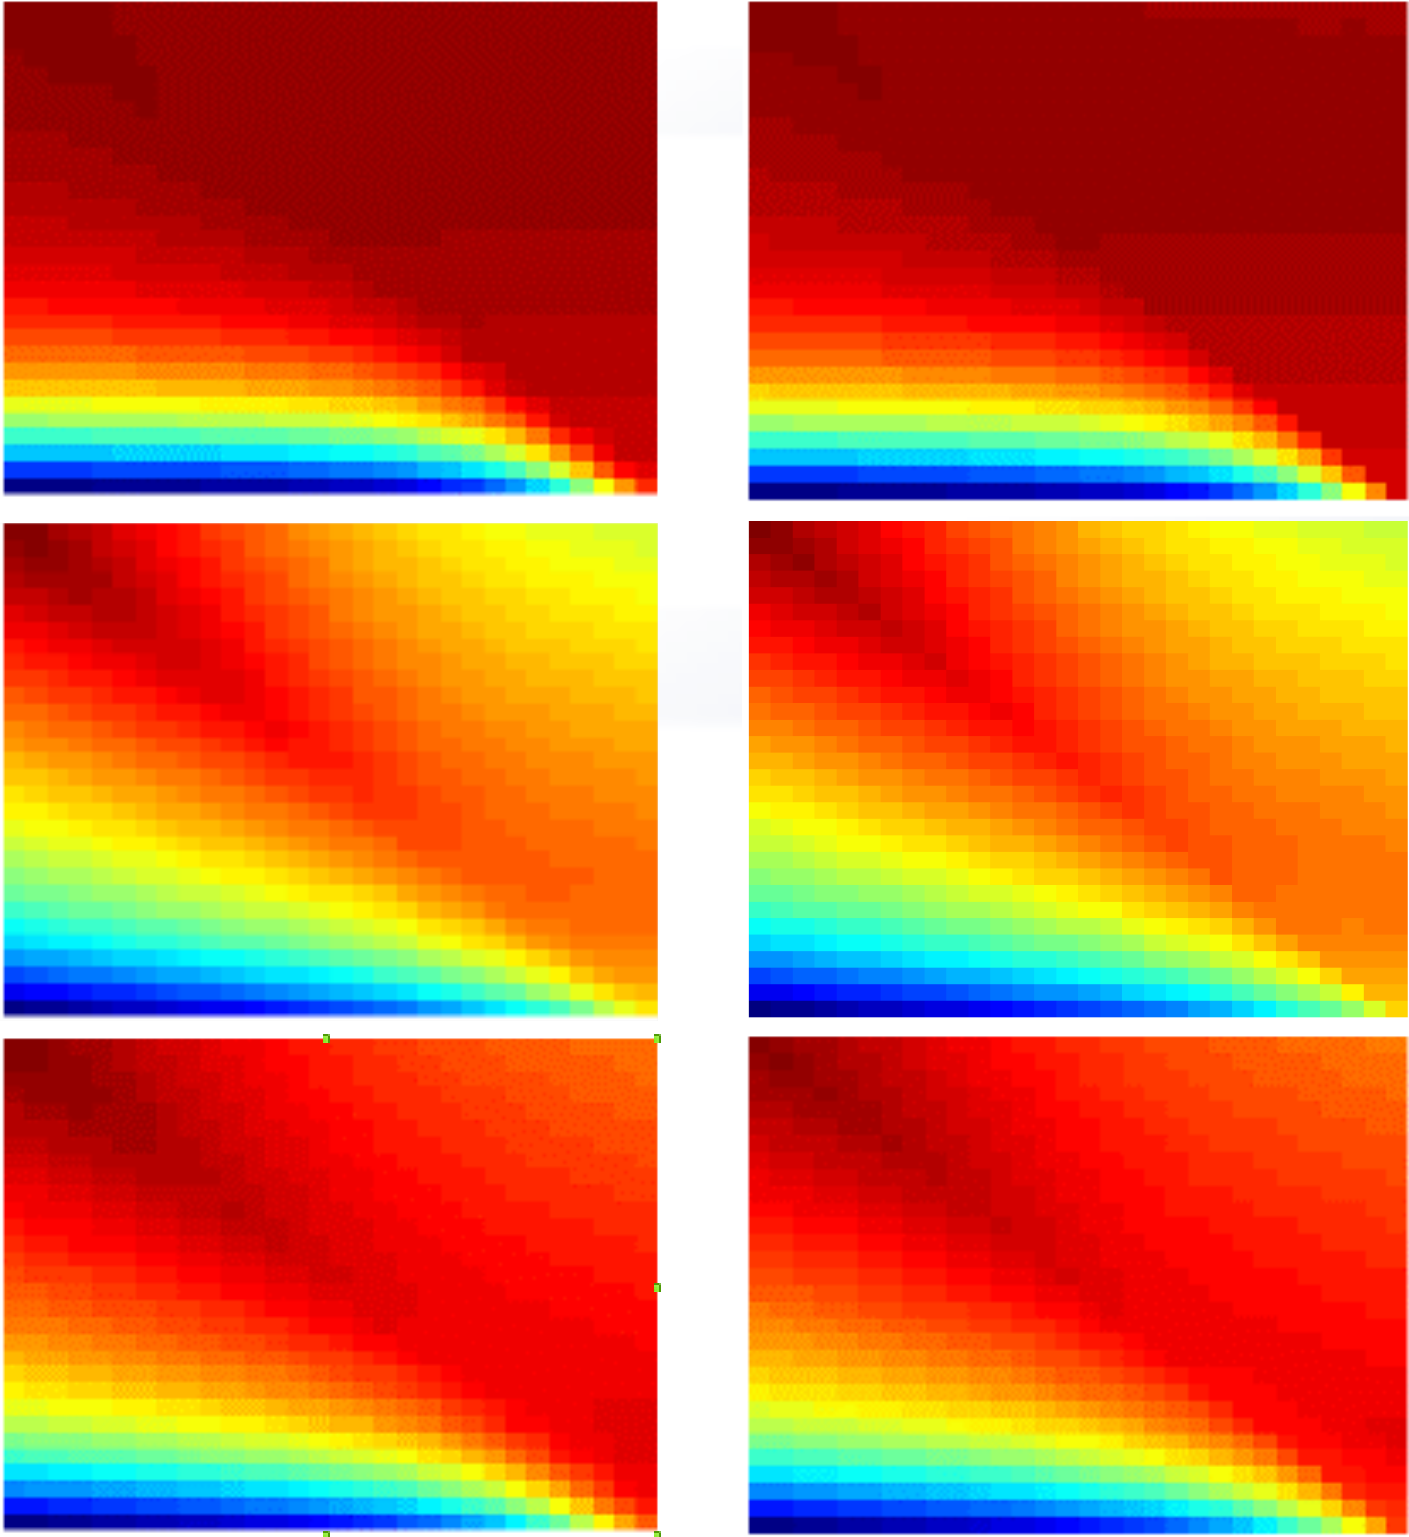
\includegraphics[width=1.5in]{projects/2.3.3-MathLibs/2.3.3.14-ALExa-ForTrilinos/tasmanian-gpu}
        \caption{\label{fig:tasmanian-gpu}Tasmanian approximation (right) of neutrino capacities (left).}
\end{figure}

{\bf ForTrilinos:}
Figure~\ref{fig:fortran_ioc} illustrates a new Inversion-of-Control~(IoC)
implementation in ForTrilinos. The new approach allows Fortran users to define
an operator by using a derived type on the Fortran side, and use Trilinos
algorithms, e.g. Krylov solvers, to solve the linear system with that operator.

\begin{figure}[htb]
    \centering
    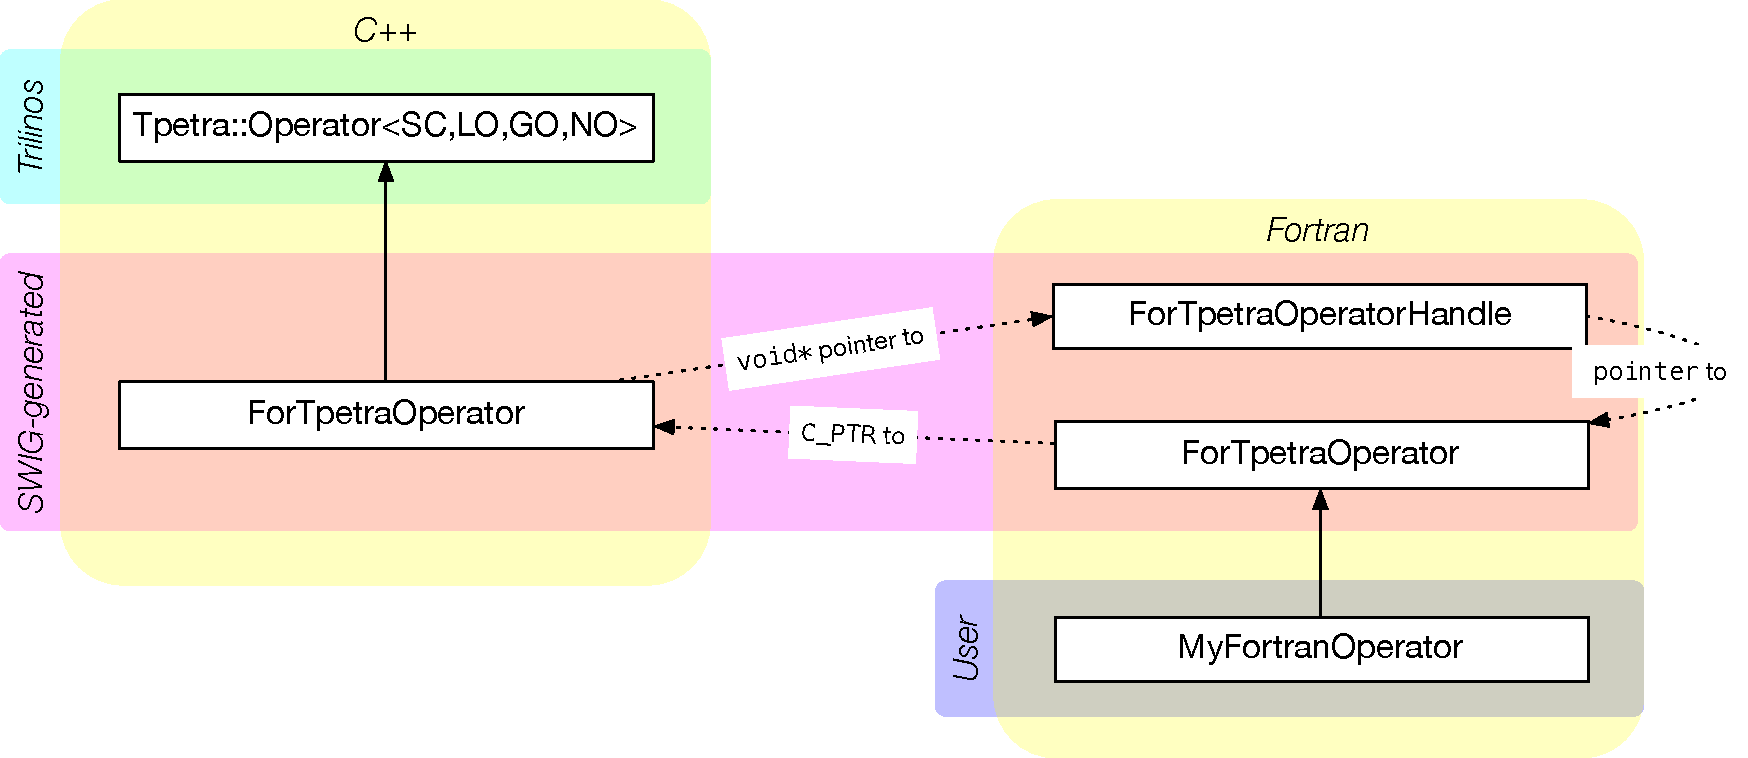
\includegraphics[scale=0.8,width=6in]{projects/2.3.3-MathLibs/2.3.3.14-ALExa-ForTrilinos/ForTrilinos_ioc}
    \caption{\label{fig:fortran_ioc}The proposed Inversion-of-Control approach
    allowing Fortran applications to define operators on Fortran side while
    still using ForTrilinos types.}
\end{figure}

This approach allows the user callback functions to interact with native Fortran
types and ForTrilinos class wrapper types. In the same vein, users would not
have to manually pass \texttt{type(C\_PTR)} instances into and out of the
callback function, as the C++ Fortran conversions can be tedious and
error-prone, which indeed is the motivation for using SWIG to generate
ForTrilinos.  Another important feature is that it allows the application code
to extend Trilinos without having to generate any new interface code, either by
hand or using SWIG. In other words, the Fortran end user should not have to know
C++ or SWIG.

%----------------------------------------

\paragraph{Next Steps}

\indent

{\bf ArborX:} Continue performance engineering campaign and extend to
distributed search capabilities and communication and deploy in a variety of
applications.

{\bf DTK:} Support parallel-in-time coupling in the ExaAM project for
simulations of metal powder bed additive manufacturing.

{\bf Tasmanian:} Work will continue with the development of mixed precision
algorithms for fast surrogate evaluations and integratinv the capability within
the ExaStar project.

{\bf ForTrilinos:} the next efforts will include
\begin{enumerate}
  \item \textbf{Provide wrappers for more libraries:} ForTrilinos will continue
    efforts to increase the number of wrapped Trilinos libraries. The scheduled
    release of the next phase of the project will include libraries
    corresponding to nonlinear solvers, such as NOX.
  \item \textbf{Integrate developed capabilities into applications:} E3SM-MMF
    is an Earth system model development and simulation project. It relies on
    Trilinos for its implicit capabilities. The ForTrilinos project will
    integrate the developed nonlinear solver with IoC into E3SM-MMF to provide
    path forward to heterogeneous stack.
  \item \textbf{Provide interfaces for heterogeneous platforms:} ForTrilinos
    will develop support for heterogeneous memory through providing access to
    Kokkos-based interfaces in Trilinos. This will allow full exposure to
    Trilinos capabilities targeting Exascale machines.
\end{enumerate}

%----------------------------------------
